\documentclass{article}
\usepackage[T1]{fontenc}
\usepackage{lmodern}
\usepackage[usenames,dvipsnames,table]{xcolor}
\usepackage{pdflscape}
\usepackage{amsmath}
\usepackage{amsthm}
\usepackage{amssymb}
\usepackage{longtable}
\usepackage{booktabs}
\usepackage{lastpage}
\usepackage{multirow}
\usepackage{longtable}
\usepackage{fancyhdr}
\usepackage{color}
\usepackage{listings}
\usepackage{minted}
\usepackage{pgffor}
\usepackage[backend=biber,style=numeric-comp]{biblatex}
\addbibresource{myref.bib}
\lstset{
basicstyle=\small\ttfamily,
keywordstyle=\color{Blue},
commentstyle=\color{OliveGreen},
numbers=left,
numberstyle=\scriptsize\ttfamily,
frame=tbrl,
}
\fancypagestyle{plain}{%
\fancyhf{}
\chead{Gesture based paint}
\rhead{\tt ad3180, ak3682}
\cfoot{Page~\thepage{}~of~\pageref{LastPage}}
}
\pagestyle{plain}
\usepackage{tikz}
\usetikzlibrary{arrows}
\usetikzlibrary{calc}
\usetikzlibrary{trees}
\usetikzlibrary{shapes}
\usetikzlibrary{shapes.symbols}
\usetikzlibrary{shapes.misc}
\title{Final Project\\ Gesture based paint system \\ \large Visual Interface COMSW 4735 Spring 2015}
\author{Angus Ding {\tt ad3180}\\ Ayaka Kume {\tt ak3682}}
\begin{document}
\maketitle
\tableofcontents
\clearpage
\section{Introduction}
\subsection{Purpose of this project}
    In this experiment, we will be implementing a system that allows the user to paint on the screen using intuitive gestures instead of the mouse. 
    Instead of using any specific draw pad or other device, we will implement the system using a simple white paper, a webcam, and a light source. 
    Without any tactile input, we are going to rely on visual inputs to determine the gesture and the position of user's hand in real-time. 
    The challenging part about this project is how to define the natural gestures that human use to indicate the drawing on a  blank paper, and how to recognize them using pure visual signal processing. Because the system only rely on the visual input, this project is perfectly suitable as an example of a visual interface. 
\subsection{Previous work}
    EnhancedDesk\cite{a} is a two handed drawing system using infrared camera. Left hand and right hand have the different role.  Isard, Michael, and John MacCormick implemented a vision based drawing package to demonstrate the hand tracking method\cite{b}.
\subsection{Program features}
The user will be given a device that consists of a white paper(or a whiteboard), a webcam that looks down from above, 
and a light source that projects light onto the paper from a non-perpendicular angle.
The distance between the webcam and the paper, the paper and the light source, and the angle of the light source are all fixed. On the bottom of the paper will be some color blocks which represent a palette, and possibly some symbols which represent the drawing tools that the user can choose. The user can simply touch the color blocks to choose the color, and touch the tool symbols to choose the painting tool he or she wants to use. On the same time there will be a program on the computer screen which shows the canvas on which the user draws. 
To draw a picture, the user can use the most intuitive gesture -- use the index finger like a pen. 
Touching the paper with the index finger means to draw, while moving the finger without touching the paper means to move the pen without drawing. 
This gesture, when the user touches the palette or the symbols instead of the empty area, means to select the color or the tool instead of drawing. 
For convenience, we will also define an erase gesture, which is a palm facing downwards with the four fingers stretching straight. This gesture is easy to use, and suitable for the semantic of erase, because it is the movement one will use to wipe something away from a surface.  
\subsection{Domain engineernig}
Fig.\ref{fig:1} shows the setting of our device. The height from the camera to the paper canvas is 54 cm. The camera looks down so that we can convert the coordinate of the fingertip to the canvas coordinate easily. The canvas on the paper is 19cm by 14cm. We set all of back ground as white in order to detect hands easily. We use the webcam, logicool carl zeiss tessar. We use Windows7 and python 2.7. As a light source, we use handy light.
\begin{figure}
 \caption{The setting of our input device}
 \label{fig:1}
\end{figure}
\subsection{Division}
Angus Ding (ad3180) implemented and wrote a report about posture detection, shadow detection and gui part.
Ayaka Kume (ak3682) implemented and wrote a report about hand detection, fingertip detection and experiment part.
We wrote introduction and discussion together.

\clearpage
\section{Overview of the method}
To complete our system, we need three informations for each frame: the posture of the hand, the location of the fingertip and whether the user's hand is touching the paper. We will dicuss how we get these informations in the following sections. 

To implement the drawing function, the system has a drawing flag which is either true or false. The system is in the drawing state if and only if 
\begin{itemize}
\item
The posture of the hand is the ``pointing finger''
\item
The fingertip is touching the paper
\end{itemize}
If the system is in the drawing state in both the previous and the current frame, a line will be drawn from the previous location of the fingertip to that of the current one. We draw a line instead of drawing a point at each location because the movement of the user's hand is usually too fast for the frequency with which we process the frames, which makes a continuous movement of the finger draw many disconnected dots instead of a line, as might be the user's intention. If either the previous frame or the current frame is not a drawing frame, then we don't draw the line. 

The similar process is used for the erase function. The difference is that the ``erasing'' state is defined with the ``palm'' posture instead of the ``pointing finger'', and instead of drawing a line with the currently selected color, we simply draw a line with the background color, which is white by default.

To allow the user to select different color to draw, we define a ``hand down'' event. A ``hand down'' event happens if the user is not touching the paper in the previous frame and is in the curren frame. When this event happens and when the user's posture is ``pointing finger'', we check if the location of the finger point is in the predefined area of one of the colors. If it is, we change the current seleceted color to it. 

No matter what the events are, the location of the cursor is always set to the current location of the fingertip. This is important because even if the user is not currently drawing, without the cursor matching the movement of the hand the user wouldn't know where he or she should put the hand down. If we can not detect the fingertip, then we assume the user is not currently using the system, and simply does nothing about this frame. 

Now we discuss how we will reteive the three important informations of each frame. 

\clearpage
h\section{Hand detection}
Because of our settings, there are only white background, shadow and the hand in an image.
First, we detect hand using skin color. Then we detect wrist. Because there are only hand or wrist in the scene, we can get hand mask by erasing wrist region. Fig.\ref{fig:hand} shows the overview of the system. For wrist detection, we modify the method from \cite{ra11}.
All of the functions in this section is in major.py and hand\_detection.py.
\subsection{Skin color detection}
Because of our settings, there are only white background, shadow and the hand in an image.
So we detect the hand by color. We use both RGB and HSV value to detect our skin.
Because both of our team mates are East Asian, we tried skin detection only for East Asian people.
In particular, we define skin color pixel as:
\begin{itemize}
  \item its Red value is larger than Blue value
  \item its Red value is larger than Green value
  \item its Value (HSV) is smaller than 73 \%
  \item its Saturation is larger than 30 \%
 \end{itemize}
Also we mask where outside of the canvas.
\subsection{Hand detection}
Then we have to extract only hand region. If there are long arms, we may not classify the gesture correctly. We modified the method introduced by \cite{ra11}. The method is first detect the skin region by color (HSV), and then detect the wrist end. Wrist end is detected by the simple method as follows:
Fig.\ref{fig:handim} shows the image of the hand. 
However, the wrist detection does not work well because the paper assumes the hand gesture as spray hand and so the palm is always the widest. 
In our case, palms are not fully opened so it is difficult to detect hand region as it is. 
So we rotate the image along the axis so that we can assume the wrist is always 'up' side and the most left or right part tend to be the palm region.
Fig.\ref{fig:handex}  can detect wrist by our method but not the proposed method. In this case, the proposed method detects the wrist side correctly, but it will calculate slope with either
wrist (blue dot) or fingertip (near yellow dot). Then proposed method does not work.
Even though we improve the method, sometimes the skin detection fails and the hand become smaller of the palm is too small to be a widest length, in that case, we simply extract 1/4 of the all of the region.
\subsection{Orientaiton of the hand}
We want to detect the orientation of the hand in order to use training data, or detecting hand region.
In our program, majoraxis.py has this function.
We define the orientation of the hand as the angle of the axis of least second moment.\par
The input is the binary image of skin region.
Axis of least second moment minimizes E, the sum of the distance from all points to the line. That is,
$$E = \int \int r^2 b(x,y) dxdy$$
where $r$ is a distance from b(x,y) to the axis and b(x,y) = 1 when a pixel (x,y) belongs to the object, otherwise 0.
Let the axis be $x\sin{\theta} - y\sin{\theta} + \rho = 0$.
Distance of point (x,y) from axis is:
$$r = |x\sin{\theta}-y\cos{\theta}+\rho|$$.
Thus minimizing $E$ means minimizing
$$E = \int\int (x\sin{\theta}-y\cos{\theta}+\rho)^2 b(x,y)dxdy$$
Because $\partial E / \partial \rho = 0$, we get
$$A(x_c \sin{\theta} - y_c \cos{\theta} + \rho) = 0$$
where $A$ is an area of the object and $(x_c,y_c)$ is center of the object.
This means, the axis should pass the center point of the object.
Then, we shift the coordinate system in order to set the center point as origin.
That is, 
$x'= x - x_c, y' = y - y_c$.
Because this line should pass the origin, the line can be represented as
$x'\sin{\theta}-y'\cos{\theta}$
So, $$E = a \sin^2{\theta} - b\sin{\theta}\cos{\theta} + c\cos^2{\theta}$$.
Where $a = \int\int (x')^2 b(x,y) dx'dy', b = 2\int\int x'y' b(x,y) dx'dy', 
c = \int\int (y')^2 b(x,y)dx'dy'$.\par
Because $\partial E / \partial \theta = 0$, we get
$$(a-c)\sin{2\theta} - b\cos{2\theta} = 0$$
Also, minimizing E means the second derivative is larger than 0.
Using these information, the orientation $\theta = atan2(b,a-c)/2$.\par
Fig.\ref{fig:mom2} shows the results of orientation detection and the rotated image.
The first column is an original image.
The second column is a translated image. First, the center point of the hand moves to the center point of the image.
The light blue line is the axis. The blue dot is the center point.\par
When we return Then the image is rotated by the angle of $-\theta$.
This shows that this axis does not depends on the small fingertip movement.
If the binary image of hand has enough amount of areas, this system can detect the angle of the hand.
If the image of hand does not have enough amount of areas, for example, it can detect only a part of fingers,
it cannot detect the angle of the hand correctly.
However, because of our settings, we always can see enough amount of hand in the target area.
\begin{figure}
 \begin{tabular}{ll}
 Original image & Rotated hands \\
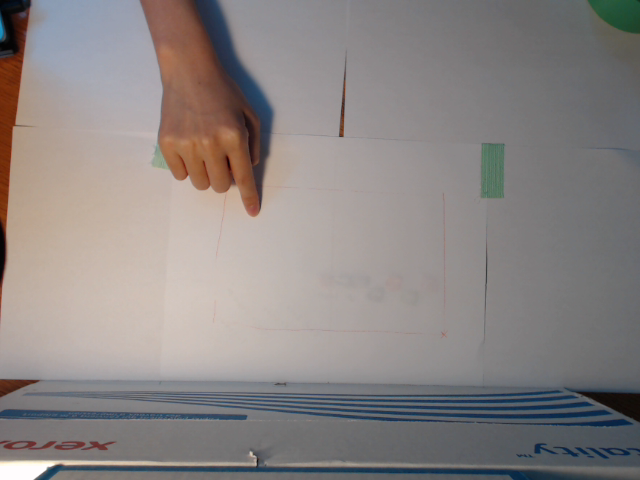
\includegraphics[width=5cm]{fig7/1-b.png} &
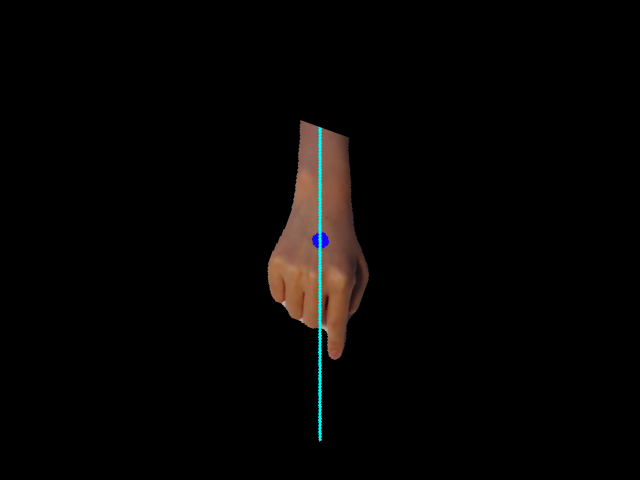
\includegraphics[width=5cm]{fig7/1-a.png} \\
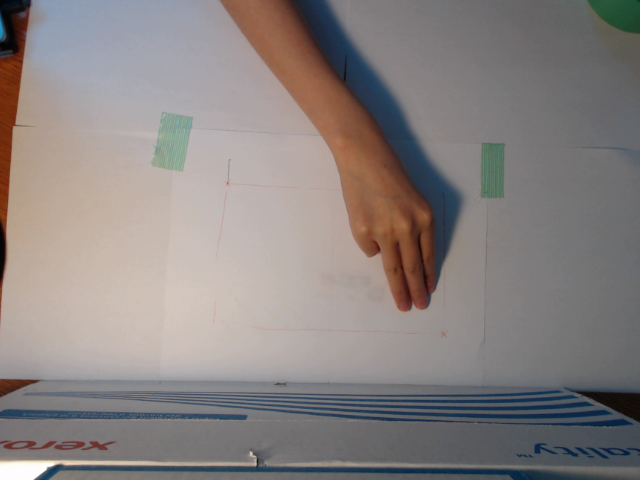
\includegraphics[width=5cm]{fig7/2-b.png} &
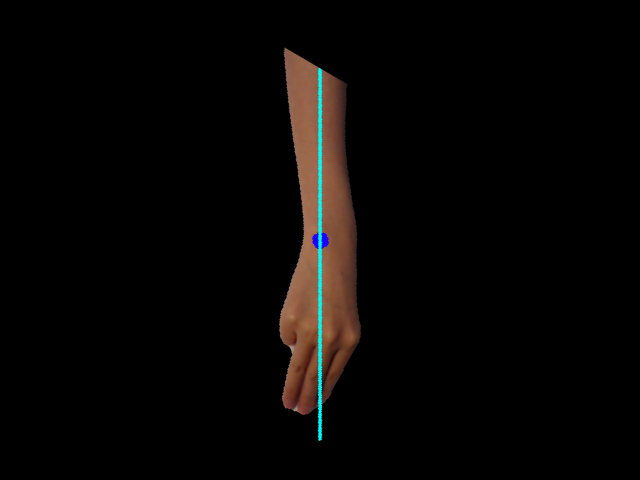
\includegraphics[width=5cm]{fig7/2-a.png} \\
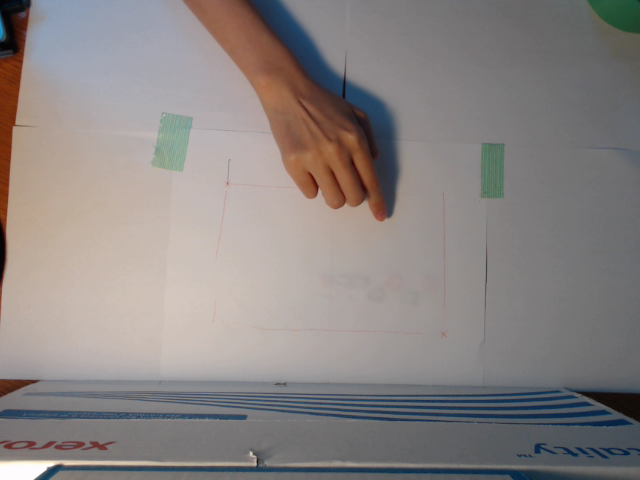
\includegraphics[width=5cm]{fig7/3-b.png} &
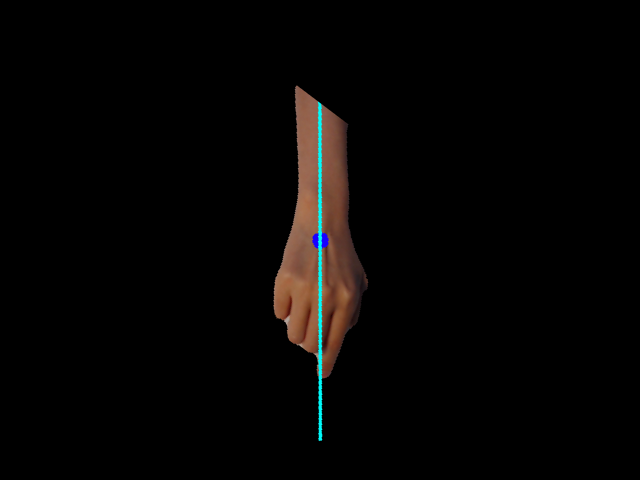
\includegraphics[width=5cm]{fig7/3-a.png} \\
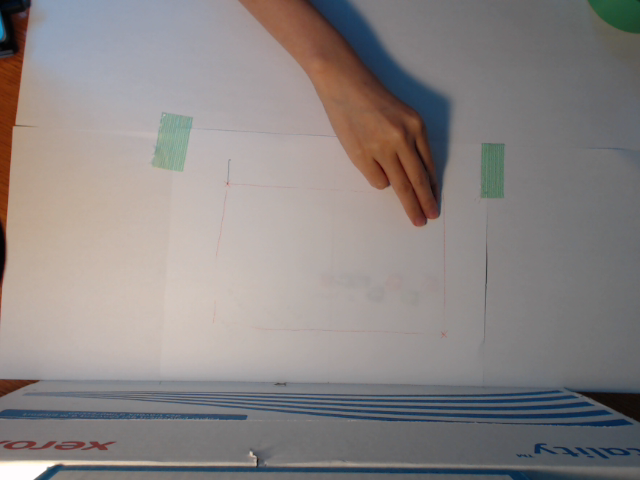
\includegraphics[width=5cm]{fig7/4-b.png} &
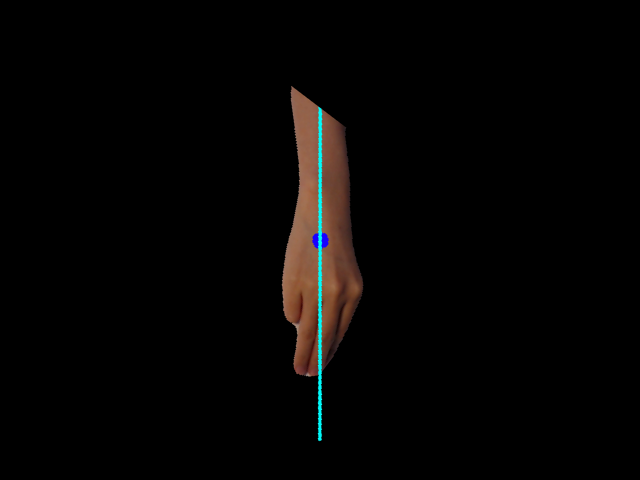
\includegraphics[width=5cm]{fig7/4-a.png} \\
\end{tabular}

 \caption{The results for orientation detection}
 \label{fig:mom2}
\end{figure}

\subsection{Result}
Fig.\ref{fig:hands} shows the results of the hand detection.
As we can see, the hands are correctly detected.

\begin{landscape}
\begin{figure}[htbp]
 \centering
 \begin{tabular}{ccccccc}
 & 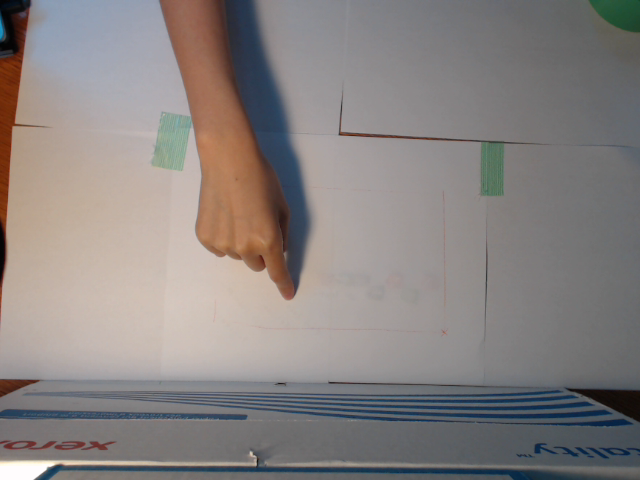
\includegraphics[width=4cm]{fig1/a.png} & $\rightarrow$ &
   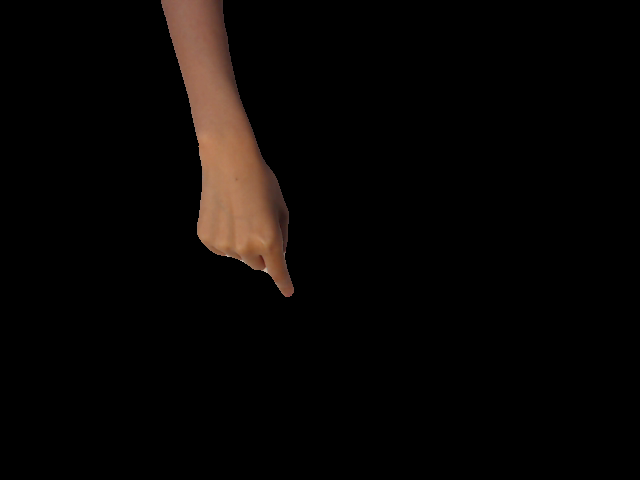
\includegraphics[width=4cm]{fig1/b.png} & $\rightarrow$ &
   
\includegraphics[width=4cm]{fig1/c.png} & $\rightarrow$ \\
& & & Skin color detection & & Major Axis detection \\
 $\rightarrow$ &
   
\includegraphics[width=4cm]{fig1/d.png} & $\rightarrow$ &
   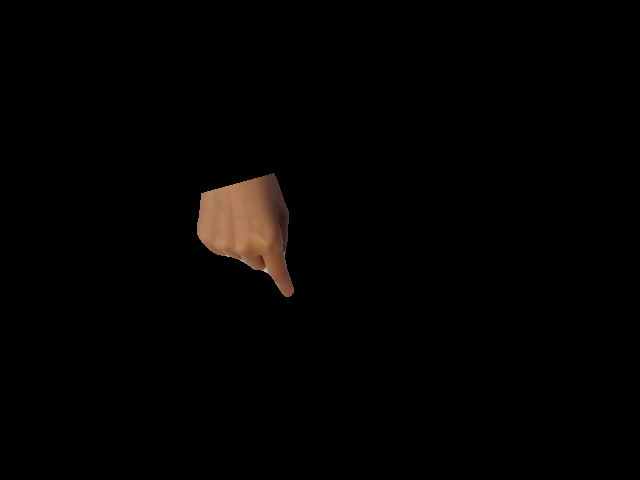
\includegraphics[width=4cm]{fig1/e.png} \\
	 & Wrist detection & & Hand mask
\end{tabular}

 \caption{Overview of hand detection}
 \label{fig:hand}
\end{figure}
\end{landscape}

\begin{landscape}
\begin{figure}[htbp]
 \centering
 \begin{tabular}{lllll}
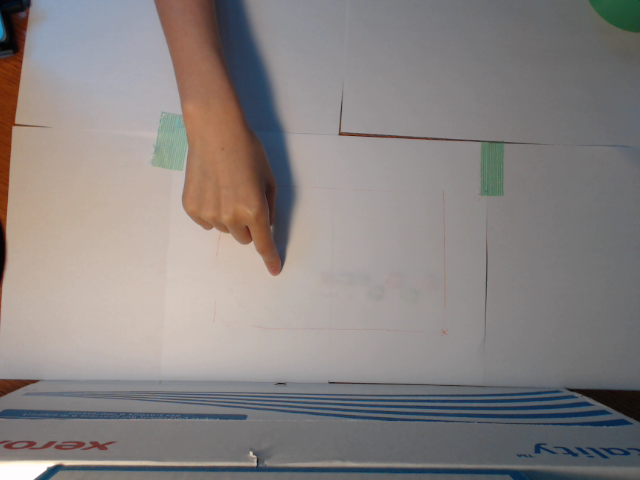
\includegraphics[width=3.5cm]{fig4/1-a.png} &
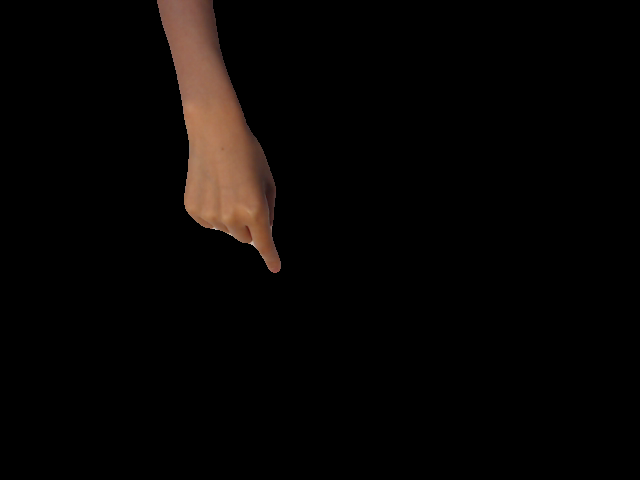
\includegraphics[width=3.5cm]{fig4/1-b.png} &
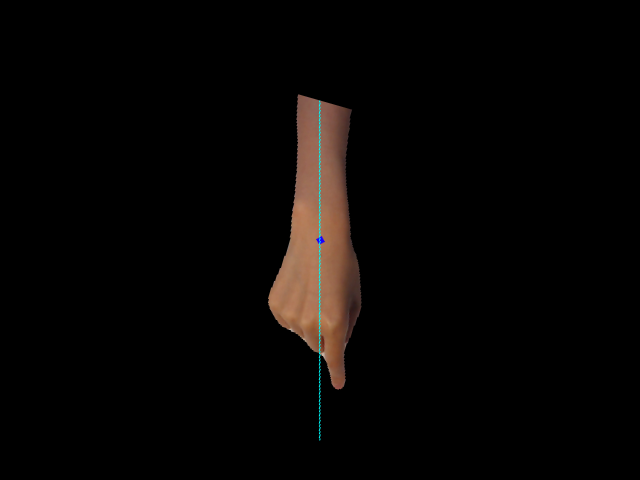
\includegraphics[width=3.5cm]{fig4/1-c.png} &
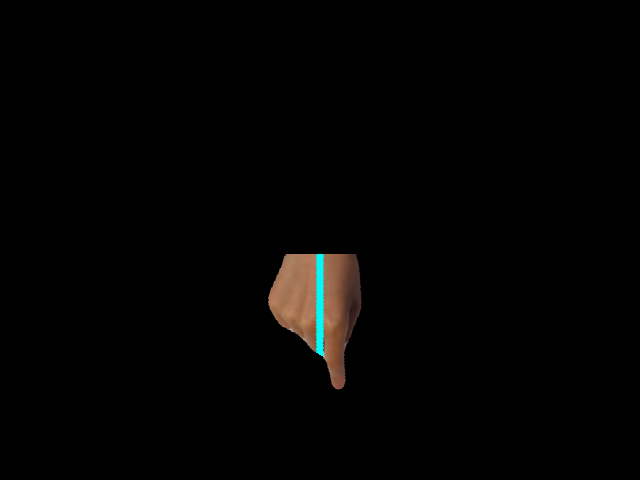
\includegraphics[width=3.5cm]{fig4/1-d.png} &
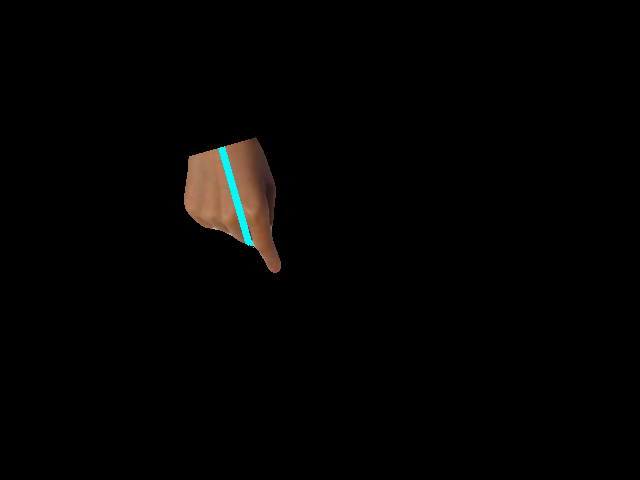
\includegraphics[width=3.5cm]{fig4/1-e.png} \\
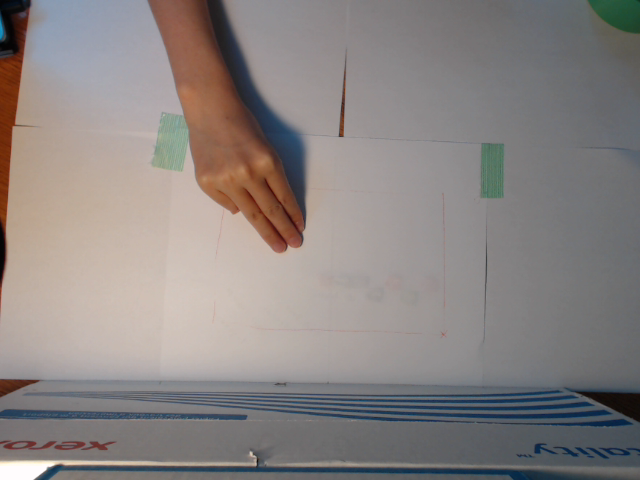
\includegraphics[width=3.5cm]{fig4/2-a.png} &
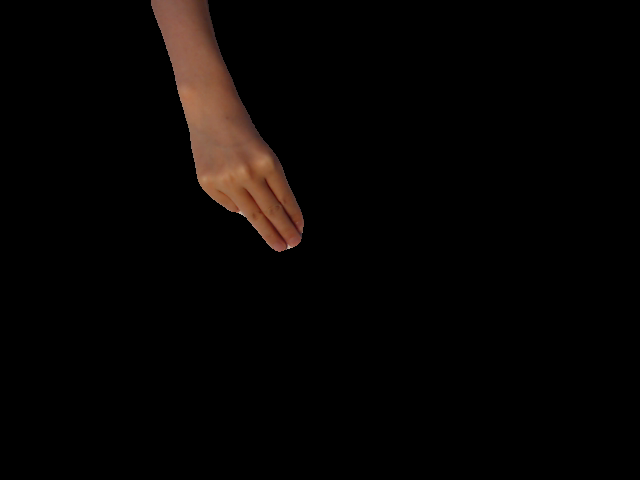
\includegraphics[width=3.5cm]{fig4/2-b.png} &
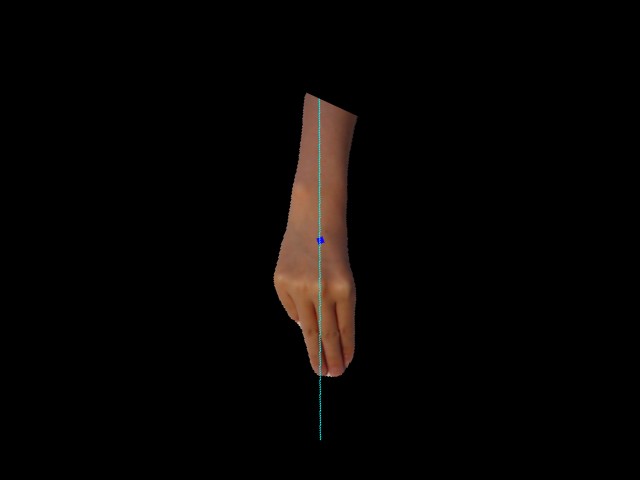
\includegraphics[width=3.5cm]{fig4/2-c.png} &
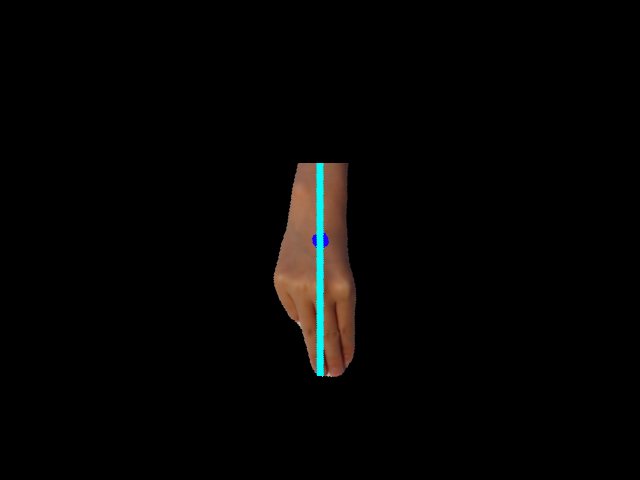
\includegraphics[width=3.5cm]{fig4/2-d.png} &
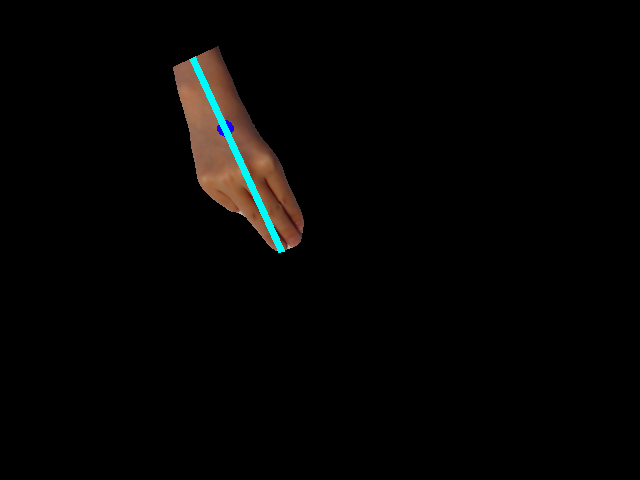
\includegraphics[width=3.5cm]{fig4/2-e.png} \\
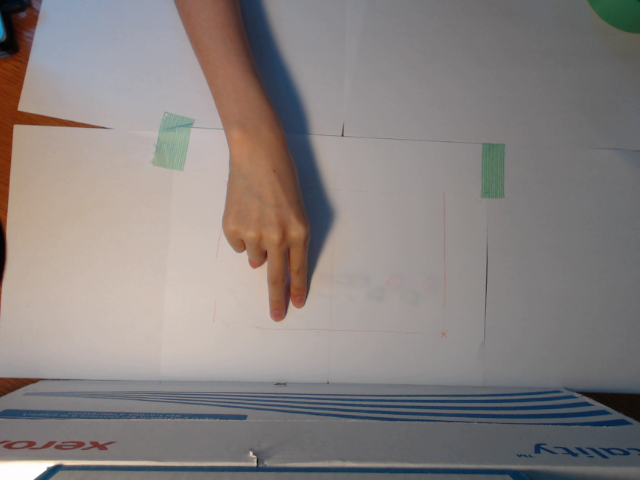
\includegraphics[width=3.5cm]{fig4/3-a.png} &
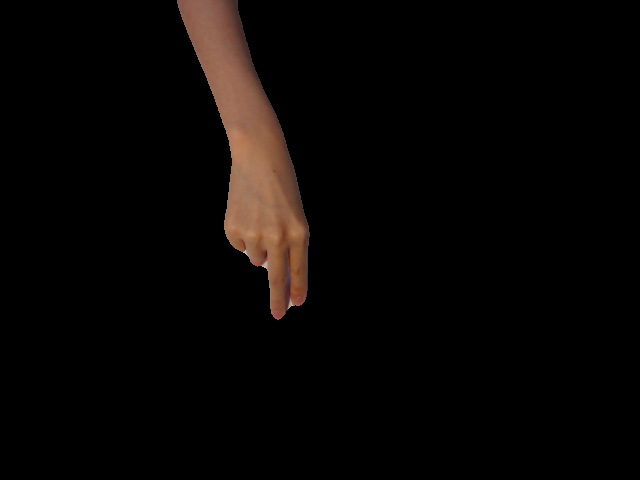
\includegraphics[width=3.5cm]{fig4/3-b.png} &
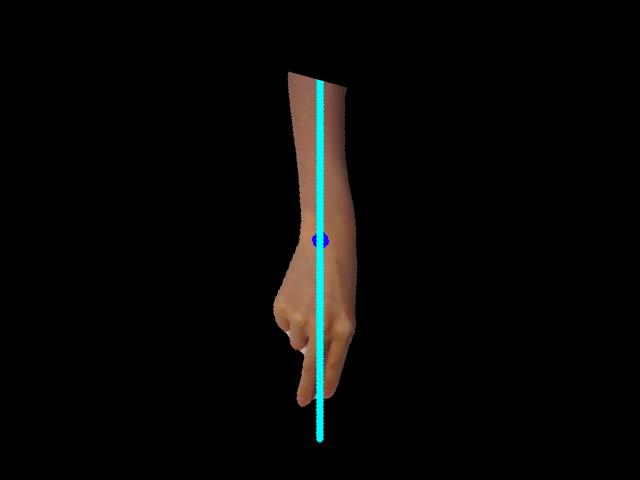
\includegraphics[width=3.5cm]{fig4/3-c.png} &
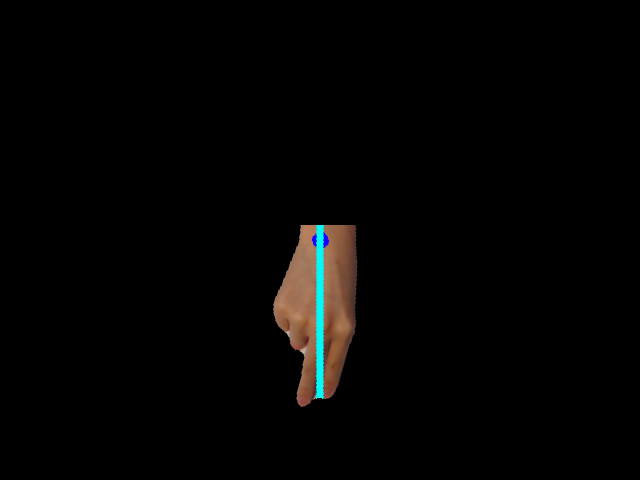
\includegraphics[width=3.5cm]{fig4/3-d.png} &
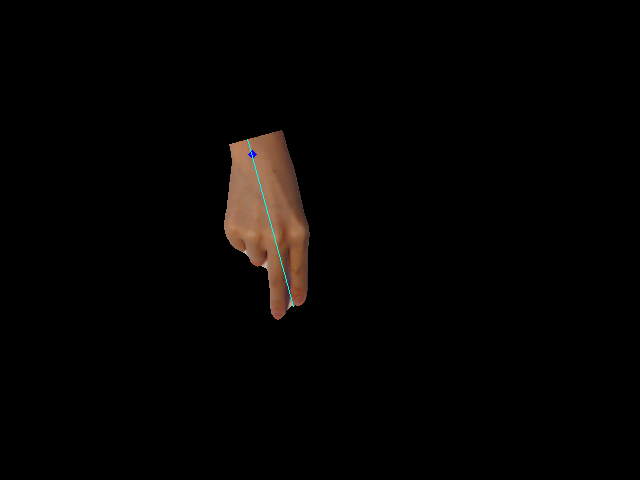
\includegraphics[width=3.5cm]{fig4/3-e.png}
\end{tabular}

 \caption{The results of hand detection}
 \label{fig:hands}
\end{figure}
\end{landscape}

\clearpage
\section{Posture recognition}

\clearpage
\subsection{Fingertip detection}
In order to draw points using finger information, we have to detect the location of the fingertip.
If the gesture is 'draw (one finger)', we detect the fingertip of the index finger. 
If the gesture is 'erase (three fingers)' or 'move (two fingers)', we detect the fingertip of the middle finger. \par
We assume the fingertip is the further point from the center of the mass and also not the wrist side.
Our environment allows us to assume the wrist side is always top of the image, we simply find the furthest point from the center of the mass among the bottom half of the mask.

This function is implemented in fingertip.py. 

Fig. \ref{fig:finger} shows the results of the finger tip detection.
This method detects the finger tip correctly when the gesture is one finger or two fingers.
When the gesture is three fingers, the method sometimes detect the location between middle finger and other fingers.
Table \ref{tb:finger} shows the result of detected finger tip when the gesture is 'three fingers'.
The error ratio is 12 \%. Fig. \ref{fig:errorfinger} shows the examples of failure. As we can see, it fails when the hand is not on the canvas. This would cause about 10 pixels error in video image and cause about 20 pixels error in canvas. This is about 3\% of the average length of the canvas.

\begin{table}
 \caption{The result of three fingers' finger tip detection}
 \label{tb:finger}
 \begin{tabular}{|c|c|}
 \hline
 The location of the result &  \\ \hline
 Index finger & 0(0\%) \\ \hline
 Between index finger and middle finger & 1(0\%) \\ \hline
 Middle finger & 124 (87\%) \\ \hline
 Between middle finger and third finger & 12(8\%) \\ \hline
 Third finger & 6(4\%) \\ \hline
 Total & 143 \\ \hline
 \end{tabular}
\end{table}

\clearpage
\section{Determine if the finger is touching the paper}
It is difficult to determine whether the finger touches the paper solely with the image taken from the direct above. As such, we use a light source to project the shadow of the hand onto the side of the hand. Suppose the light source is set to have angle $\theta$ from the vertical line, and the fingertip is at height $h$, then the distance between the fingertip of the shadow and the x-coordinate of the real fingership is $d = h \tan(\theta)$. So, if $\theta is not $0$, we can find $h$ with $h = d \cot(\theta)$. Or, since we only care if the finger is touching the paper or not, we can set a threshold $d_{th}$ such that we can assume the finger is touching the paper if and only if $d < d_{th}$. 

This method thus requires the detection of the shadow and its fingertip. We detect the shadow with the similar method for hand detection: using color filters and HSV filters. The actually condition we use are as follows:
\begin{itemize}
\item
$R < 107.1 $\\
\item
$G < 86.7 $\\
\item
$B < 120.6 $\\
\item
$V < 100.8 $\\
\end{itemize}•
, where $R, G, B$ are the red, green and blue values respectively, and $V$ is the value in HSV representation. 

To find the fingertip of the shadow, we can not use the same method proposed for finding the real fingertip because a large portion of the shadow is blocked by the hand when the hand is close to the paper, thus the center of mass of the shadow can be greatly affected.  Instead, we simply assume that the fingertip is always pointing down, and find the pixel of the shadow that has the lowest y-coordinate. Because we set the ligth source to be at the lower left corner of the screen, the shadow of the hand will always be at the upper-right side of it. Under the assumption that the finger is always pointing down, we ignore all the shadow pixels that are to the left and lower than the fingertip to reduce  noise. Further more, since we only care if the fingertip is touching the paper, we can ignore all the shadow pixels that are too far away from the real fingertip. So, we only find the shadow fingertip in the region of $\{(x,y): x_{finger}<x<x_{finger}+40, y_{finger}<y\}$. 

Finally, we have to decide the threshold for the distance between the real fingertip and the shadow fingertip. This threshold is affected by the posture. When the user is posing the palm posture and is touching the paper, a larger portion of the shadow will be blocked than when the user is posing the pointing finger. So, the threshold we decided was 30 for the pointing finger and 50 for the palm. 
\clearpage
\clearpage
\section{Evaluation}
For evaluation, we measure time, error rate and the consistency of each trials.
If time is fast, it means the system is easy to operate.
If the average error is low, it means the system is accurate.
If time and average error does not change for every trial, it means the system is stable.
\par
We only evaluate about 'drawing' function because 'drawing' function is the most essential function of the system.
We evaluate this system using three tasks. Fig. \ref{task} shows three examples.
The flow of the evaluation is as follows. At first, there is a white canvas and pointer.
When the tester press 'r', it shows the sample to trace and starts timer.
User starts drawing and when he finish drawing, the tester press 'q' and timer ends.
The user do same task three times.
Time is measured by this timer. The average error is measured by the difference between the example and what he draw. The consistency is measured by the standard deviation of time and average error.
\par
To compare the results, we also testd the mouse as the input device. When we point a point in the canvas using a mouse, the pointer moves. When we drag with left click, it draws a line.\par
We used user as both of our team member.
\subsection{The average error measurement}
\subsubsection{Points}
We measure the distance between what the user draw and the nearest point of the sample.
To make the measurement easy, we devide the canvas into 4 section.
If a point the user draw is on upper left, we compare the distance with upper left point of the sample. Same as upper right, lower left and lower right.
\subsubsection{Circle}
Circle is the points which distance from the center point are radius.
We know the center point and the radius of the sample circle.
Thus we measure the absolute difference between radius and the actual difference from the center point for each points. Then we average them.
\subsubsection{Line}
We measure the distance between the actual line and sample line by comparing only 20 points of the lines. We equally sample 20 points in the lines along the vartical axis. And from the most highest points to the most lowest Points, we measure the difference of them.
Fig.\ref{linem} shows the example. Blue line is a sample line and red line is user's line. The points are sample points. Each points are measured with the points which are connected by the black line.
\begin{figure}
\begin{tabular}{|c|c|c|}
 Points & circle & line \\ \hline
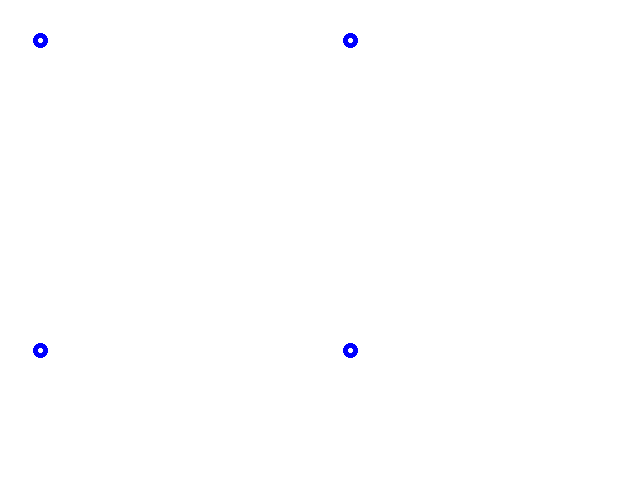
\includegraphics[width=4cm]{fig_exp/points.png} &
 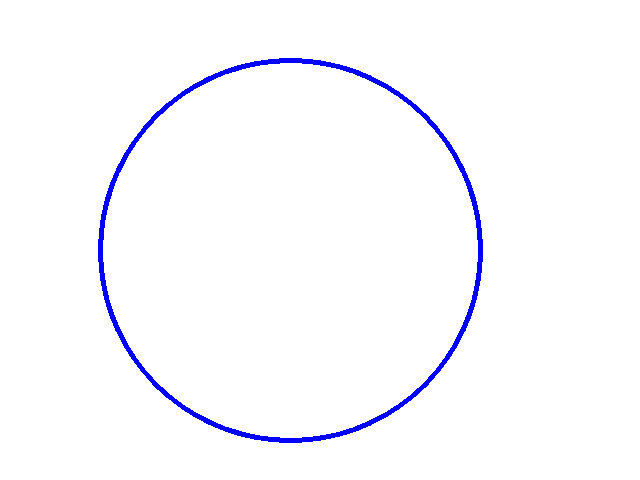
\includegraphics[width=4cm]{fig_exp/circle.png} &
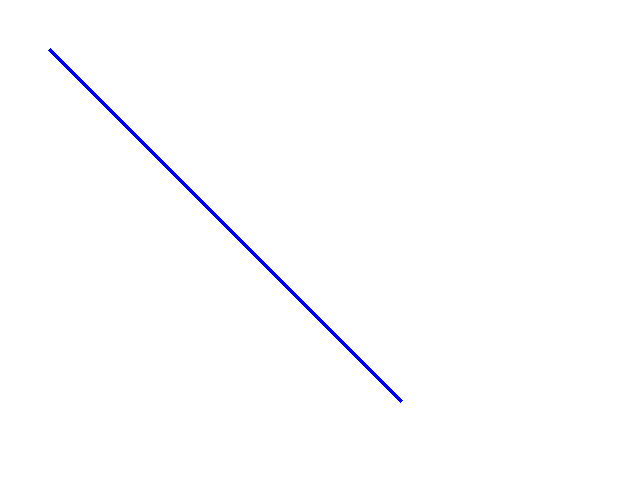
\includegraphics[width=4cm]{fig_exp/line.png}
\end{tabular}

 \caption{Three tasks}
 \label{task}
\end{figure}

\begin{figure}[htbp]
 \centering
 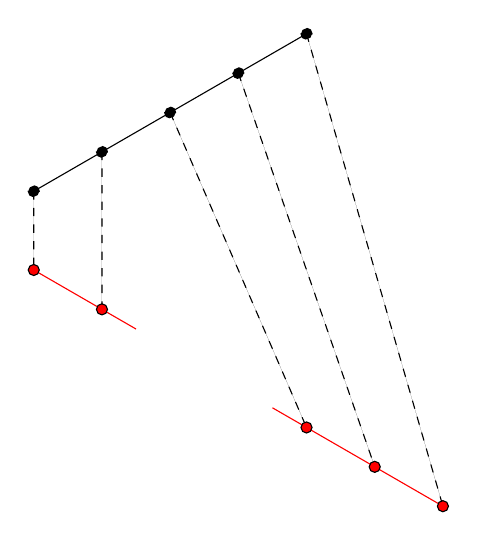
\begin{tikzpicture}
 \draw (0, 0) -- ++(30:4);
 \draw[red] (0, -1) -- ++ (-30:1.5);
 \draw[red] (0, -1) + (-30:3.5) -- ++(-30:6);
 \draw[dashed,fill] (0, 0) circle (2pt) -- (0, -1);
 \draw[dashed,fill] (0, 0) + (30:1) circle (2pt) -- ($(0, -1) + (-30:1)$);
 \draw[dashed,fill] (0, 0) + (30:2) circle (2pt) -- ($(0, -1) + (-30:4)$);
 \draw[dashed,fill] (0, 0) + (30:3) circle (2pt) -- ($(0, -1) + (-30:5)$);
 \draw[dashed,fill] (0, 0) + (30:4) circle (2pt) -- ($(0, -1) + (-30:6)$);
 \draw[fill=red] (0, -1)           circle (2pt);
 \draw[fill=red] (0, -1) + (-30:1) circle (2pt);
 \draw[fill=red] (0, -1) + (-30:4) circle (2pt);
 \draw[fill=red] (0, -1) + (-30:5) circle (2pt);
 \draw[fill=red] (0, -1) + (-30:6) circle (2pt);

\end{tikzpicture}

 \caption{Line error measurement}
 \label{linem}
\end{figure}


\subsection{Results}
Table \ref{tb:p2} shows the measurement results of the points task. Table \ref{tb:c1} and Table \ref{tb:c2} show the results of the circle task and the actual canvas image. Table \ref{tb:l1} and Table \ref{tb:l2} show the results of the line task and the actual canvas image. Table \ref{tb:exp} shows the standard deviation of them. In all tasks, mouse device results are better than our input device. Among three tasks, for our device performance is better in circle task. We can see the time deviation is better than the error deviation.

\begin{table}[htbp]
 \centering
 \caption{The result of the user study (points)}
 \label{tb:p2}
 \begin{tabular}{llrrr}
 \toprule
 User & Device & Trial & Time[sec] & Error [pixels] \\
 \midrule
A	&	VI	&	1	&	13.32	&	68.558	\\
A	&	VI	&	2	&	14.522	&	88.314	\\
A	&	VI	&	3	&	15.282	&	68.406	\\
B	&	VI	&	1	&	17.87	&	72.838	\\
B	&	VI	&	2	&	12.132	&	68.172	\\
B	&	VI	&	3	&	6.599	&	71.913	\\
C	&	VI	&	1	&	13.127	&	74.432	\\
C	&	VI	&	2	&	14.004	&	51.564	\\
C	&	VI	&	3	&	13.183	&	67.076	\\
A	&	VI2	&	1	&	11.856	&	63.8	\\
A	&	VI2	&	2	&	12.086	&	58.081	\\
A	&	VI2	&	3	&	18.693	&	89.614	\\
B	&	VI2	&	1	&	10.93	&	88.821	\\
B	&	VI2	&	2	&	13.809	&	104.269	\\
B	&	VI2	&	3	&	8.009	&	67.539	\\
C	&	VI2	&	1	&	18.943	&	31.226	\\
C	&	VI2	&	2	&	17.128	&	66.85	\\
C	&	VI2	&	3	&	16.892	&	87.412	\\
A	&	Mouse	&	1	&	6.716	&	4.125	\\
A	&	Mouse	&	2	&	7.444	&	10.296	\\
A	&	Mouse	&	3	&	7	&	4.634	\\
B	&	Mouse	&	1	&	8.113	&	4.746	\\
B	&	Mouse	&	2	&	6.293	&	8.115	\\
B	&	Mouse	&	3	&	6.428	&	7.388	\\
C	&	Mouse	&	1	&	5.4	&	4.989	\\
C	&	Mouse	&	2	&	5.481	&	4.768	\\
C	&	Mouse	&	3	&	5.199	&	6.603	\\
 \bottomrule
\end{tabular}

\end{table}


\begin{table}[htbp]
 \centering
 \caption{The result of the user study (circle)}
 \label{tb:c1}
 \begin{tabular}{lccc}
\toprule
 & Trial 1 & Trial 2 & Trial 3\\
\midrule
 User A (VI)&
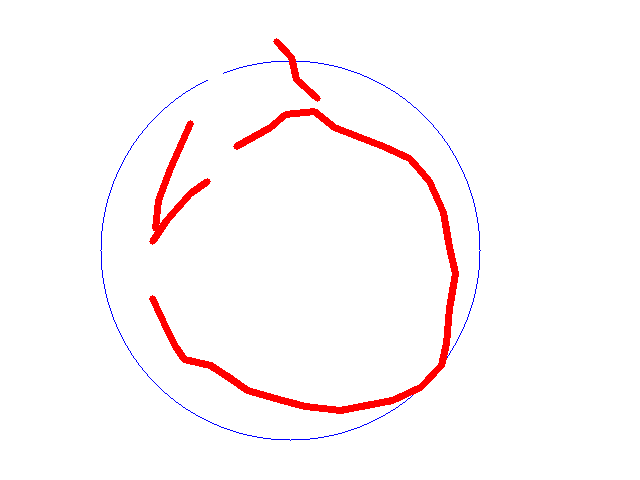
\includegraphics[width=3cm]{fig_exp/circle_Ayaka_test3_0.png} &
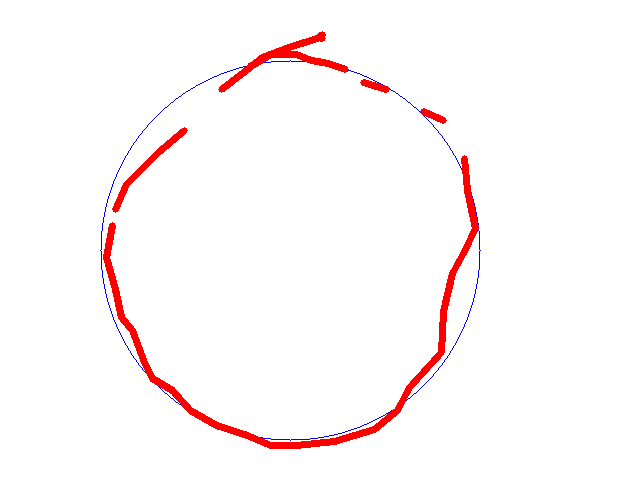
\includegraphics[width=3cm]{fig_exp/circle_Ayaka_test3_1.png} &
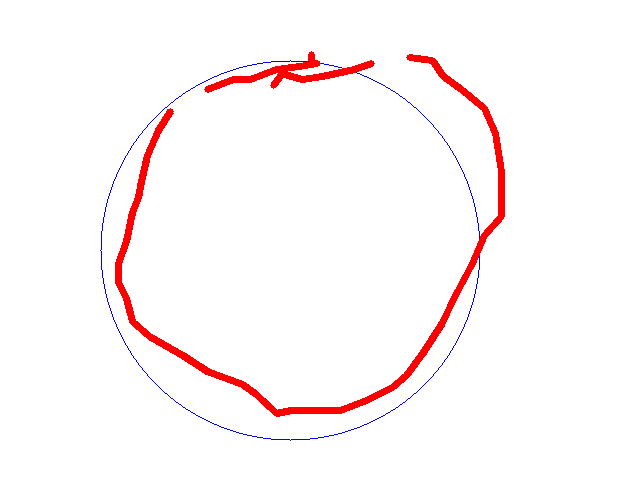
\includegraphics[width=3cm]{fig_exp/circle_Ayaka_test3_2.png} \\
\midrule
 User B (VI)&
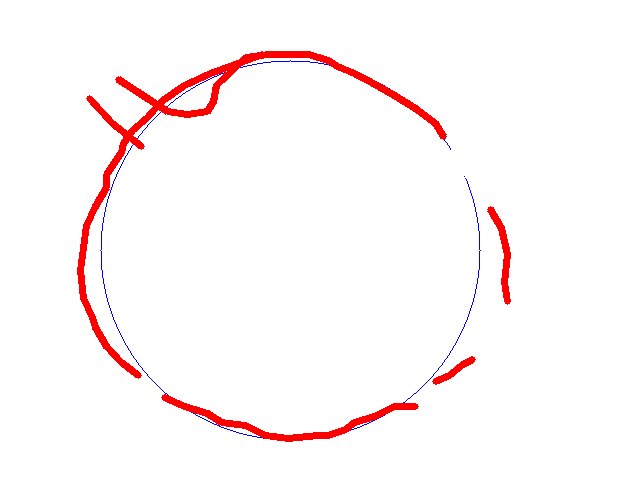
\includegraphics[width=3cm]{fig_exp/circle_Angus_test3_0.png} &
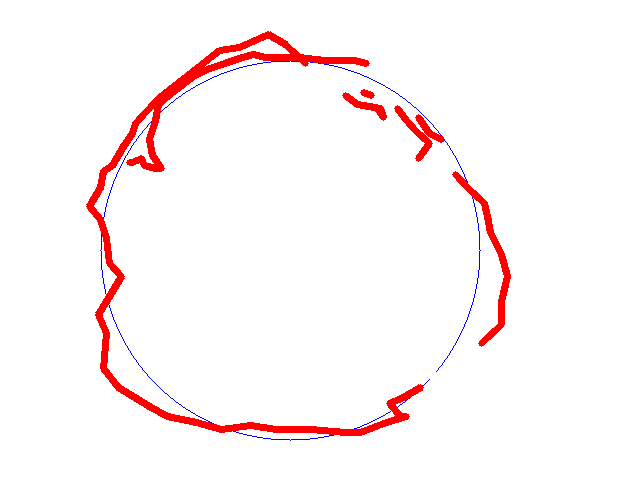
\includegraphics[width=3cm]{fig_exp/circle_Angus_test3_1.png} &
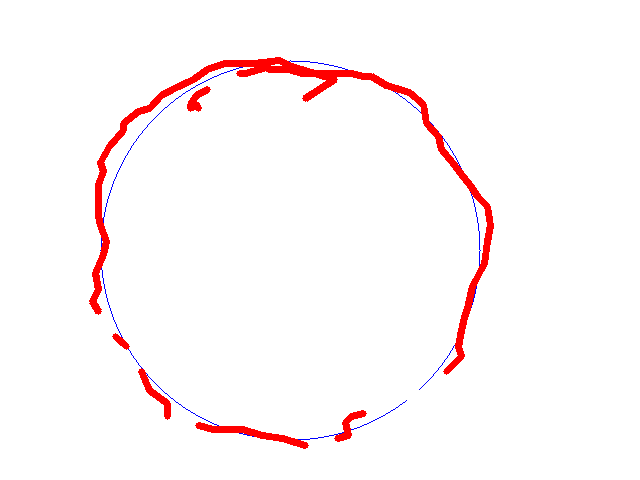
\includegraphics[width=3cm]{fig_exp/circle_Angus_test3_2.png} \\
\midrule
 User A (Mouse)&
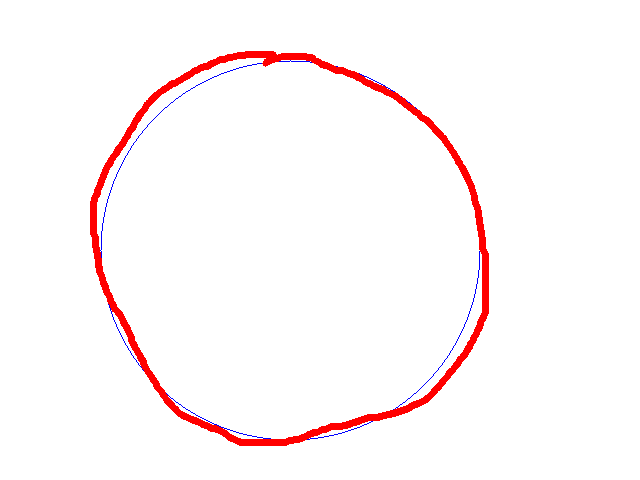
\includegraphics[width=3cm]{fig_exp/circle_Ayaka_test3_0_m.png} &
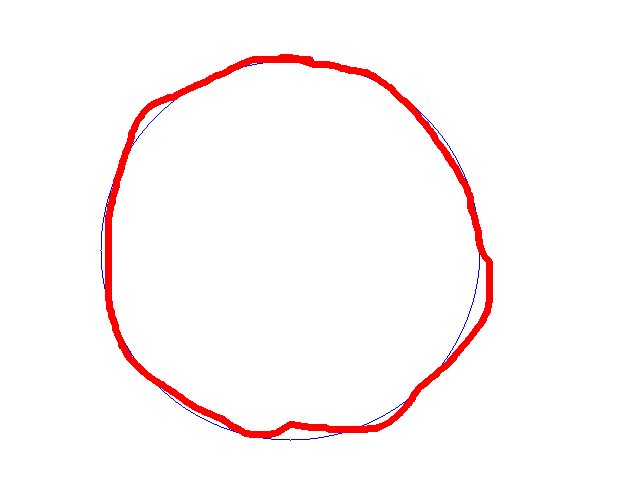
\includegraphics[width=3cm]{fig_exp/circle_Ayaka_test3_1_m.png} &
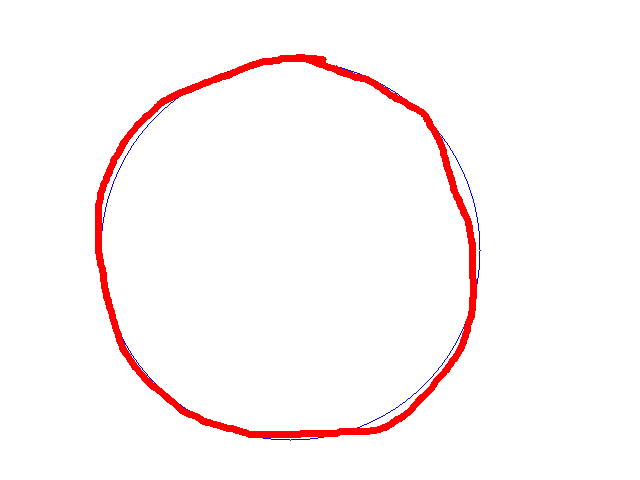
\includegraphics[width=3cm]{fig_exp/circle_Ayaka_test3_2_m.png} \\
\midrule
 User B (Mouse)&
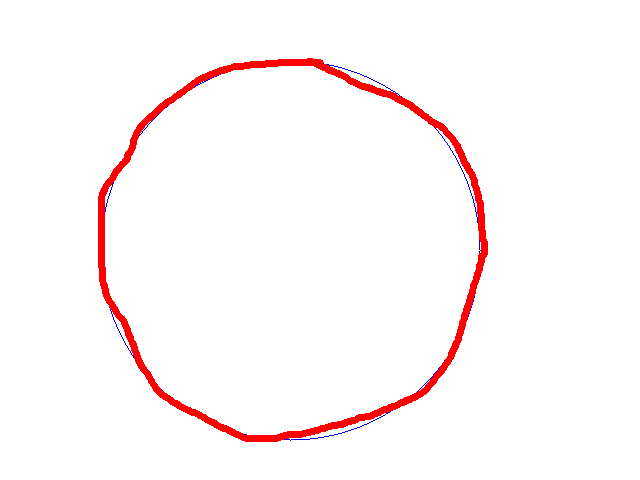
\includegraphics[width=3cm]{fig_exp/circle_Angus_test3_0_m.png} &
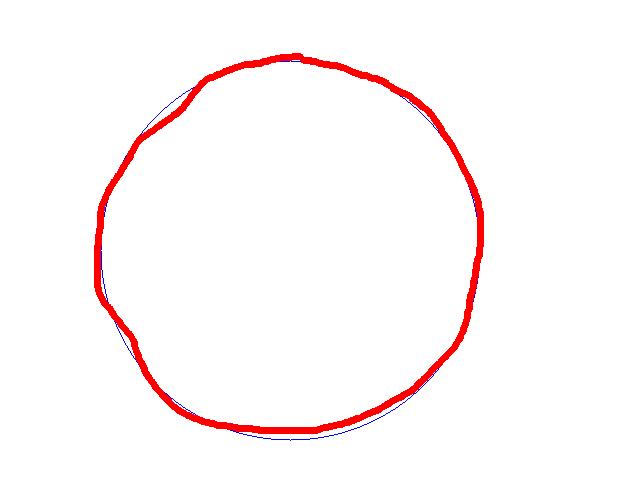
\includegraphics[width=3cm]{fig_exp/circle_Angus_test3_1_m.png} &
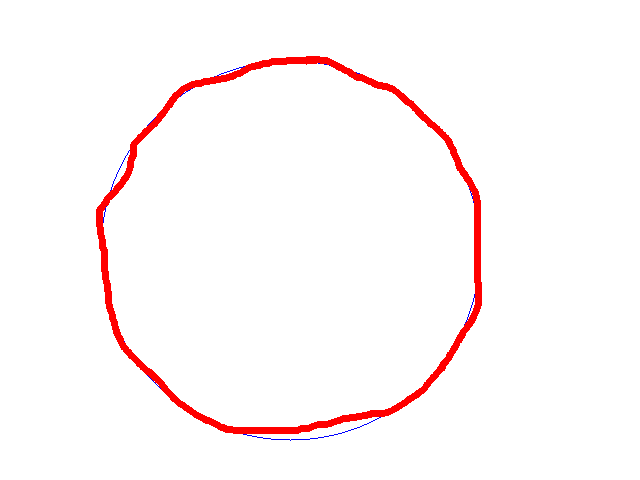
\includegraphics[width=3cm]{fig_exp/circle_Angus_test3_2_m.png} \\
\bottomrule
\end{tabular}


\end{table}



\begin{table}[htbp]
 \centering
 \caption{The result of the user study (circle)}
 \label{tb:c2}
 \begin{tabular}{llrrr}
 \toprule
 User & Device & Trial & Time[sec] & Error [pixels] \\
 \midrule
A	&	VI	&	1	&	14.507	&	12.745	\\
A	&	VI	&	2	&	17.756	&	18.283	\\
A	&	VI	&	3	&	20.314	&	17.653	\\
B	&	VI	&	1	&	8.131	&	24.242	\\
B	&	VI	&	2	&	7.84	&	14.619	\\
B	&	VI	&	3	&	7.962	&	13.559	\\
C	&	VI	&	1	&	8.433	&	46.652	\\
C	&	VI	&	2	&	10.818	&	17.856	\\
C	&	VI	&	3	&	11.376	&	10.398	\\
A	&	VI2	&	1	&	20.229	&	6.966	\\
A	&	VI2	&	2	&	17.148	&	9.991	\\
A	&	VI2	&	3	&	17.836	&	7.156	\\
B	&	VI2	&	1	&	10.819	&	12.892	\\
B	&	VI2	&	2	&	11.19	&	13.977	\\
B	&	VI2	&	3	&	12.79	&	17.879	\\
C	&	VI2	&	1	&	10.963	&	12.154	\\
C	&	VI2	&	2	&	11.597	&	7.066	\\
C	&	VI2	&	3	&	12.712	&	8.156	\\
A	&	Mouse	&	1	&	8.187	&	8.815	\\
A	&	Mouse	&	2	&	10.502	&	4.736	\\
A	&	Mouse	&	3	&	9.929	&	5.995	\\
B	&	Mouse	&	1	&	8.801	&	4.548	\\
B	&	Mouse	&	2	&	7.999	&	4.067	\\
B	&	Mouse	&	3	&	8.039	&	4.741	\\
C	&	Mouse	&	1	&	7.474	&	6.215	\\
C	&	Mouse	&	2	&	7.187	&	6.929	\\
C	&	Mouse	&	3	&	7.519	&	5.348	\\
 \bottomrule
\end{tabular}

\end{table}

\begin{table}[htbp]
 \centering
 \caption{The result of the user study (line)}
 \label{tb:l1}
 \begin{tabular}{lccc}
\toprule
 & Trial 1 & Trial 2 & Trial 3\\
\midrule
 User A (VI)&
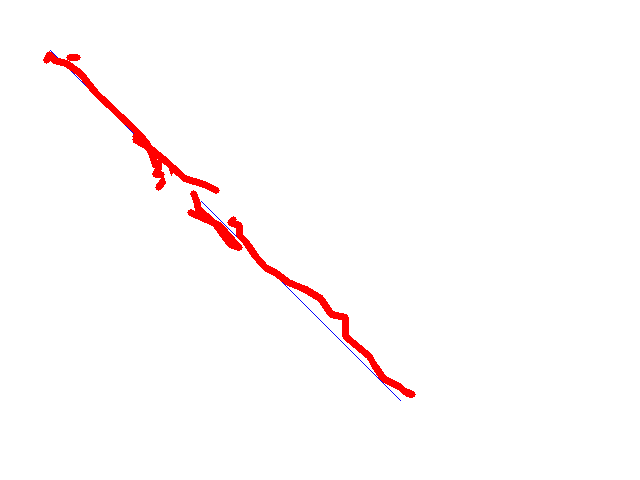
\includegraphics[width=3cm]{fig_exp/line_Ayaka_test3_0.png} &
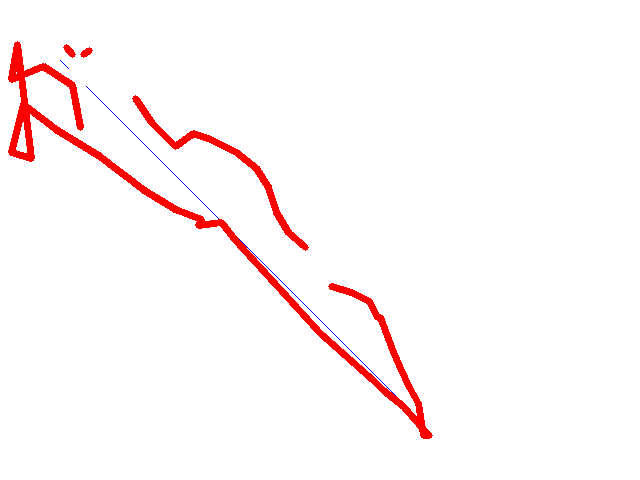
\includegraphics[width=3cm]{fig_exp/line_Ayaka_test3_1.png} &
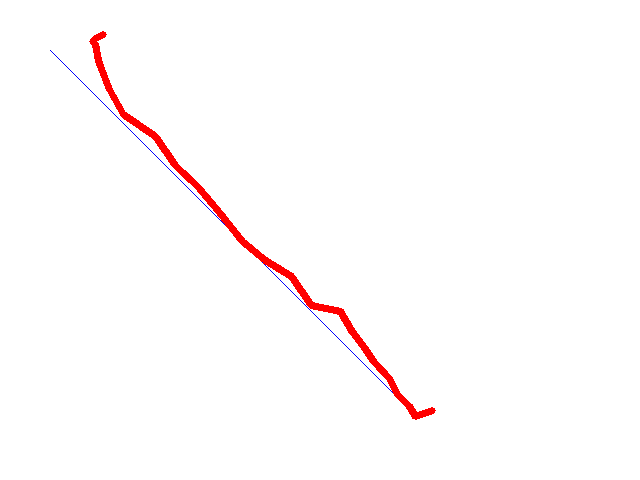
\includegraphics[width=3cm]{fig_exp/line_Ayaka_test3_2.png} \\
\midrule
 User B (VI)&
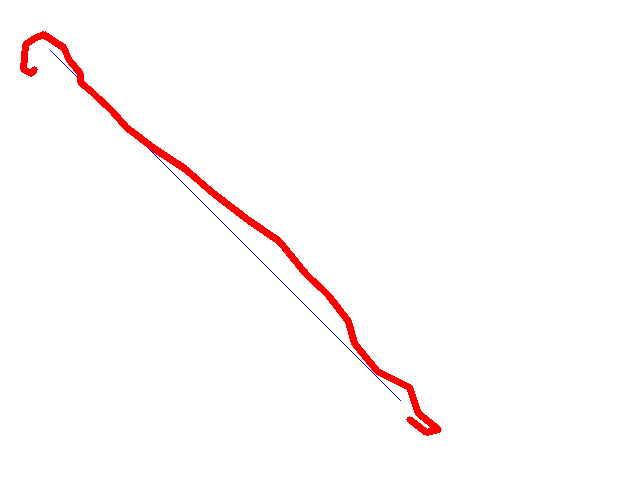
\includegraphics[width=3cm]{fig_exp/line_Angus_test3_0.png} &
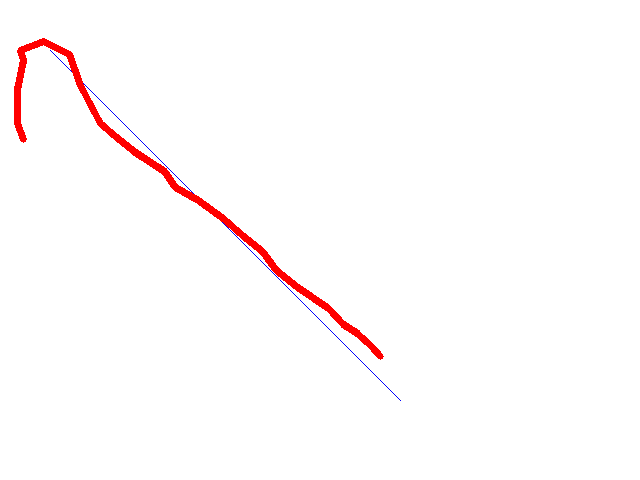
\includegraphics[width=3cm]{fig_exp/line_Angus_test3_1.png} &
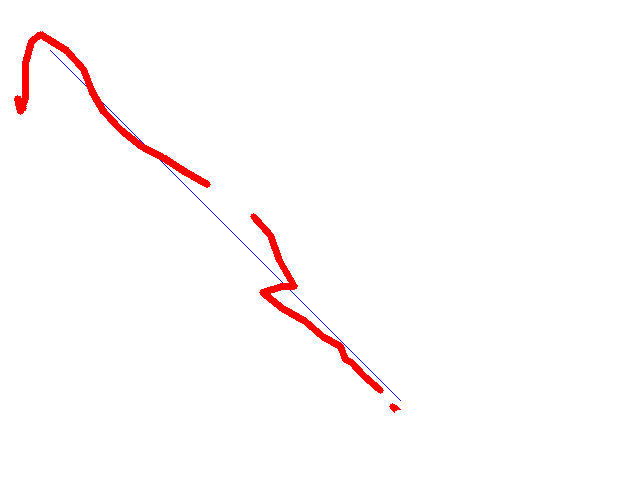
\includegraphics[width=3cm]{fig_exp/line_Angus_test3_2.png} \\
\midrule
 User A (Mouse)&
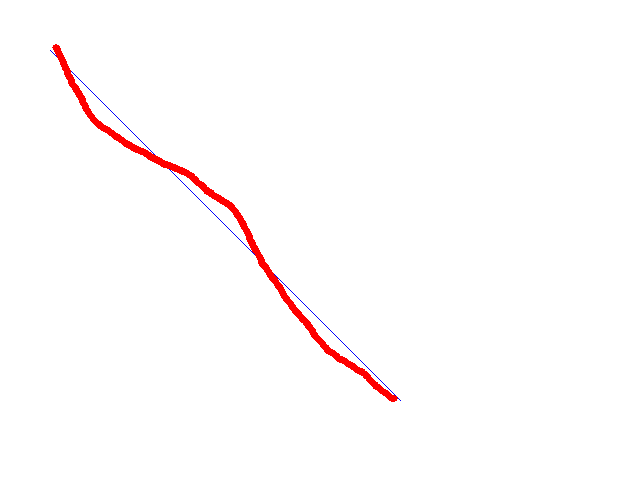
\includegraphics[width=3cm]{fig_exp/line_Ayaka_test3_0_m.png} &
\includegraphics[width=3cm]{fig_exp/line_Ayaka_test3_1_m.png} &
\includegraphics[width=3cm]{fig_exp/line_Ayaka_test3_2_m.png} \\
\midrule
 User B (Mouse)&
\includegraphics[width=3cm]{fig_exp/line_Angus_test3_0_m.png} &
\includegraphics[width=3cm]{fig_exp/line_Angus_test3_1_m.png} &
\includegraphics[width=3cm]{fig_exp/line_Angus_test3_2_m.png} \\
\bottomrule
\end{tabular}

\end{table}


\begin{table}[htbp]
 \centering
 \caption{The result of the user study (line)}
 \begin{tabular}{llrrr}
 \toprule
 User & Device & Trial & Time[sec] & Error Pixels \\
 \midrule
 A	& VI	  & 1	& 20.16	& 22.25 \\
 A	& VI	  & 2	& 14.75	& 76.46 \\
 A	& VI	  & 3	& 5.73	& 25.77 \\
 B	& VI	  & 1	& 7.76	& 39.92 \\
 B	& VI	  & 2	& 8.03	& 88.50 \\
 B	& VI	  & 3	& 10.03	& 58.27 \\
 A	& Mouse	& 1	& 4.07	& 13.87 \\
 A	& Mouse	& 2	& 5.19	& 6.53 \\
 A	& Mouse	& 3	& 4.07	& 8.01 \\
 B	& Mouse	& 1	& 3.98	& 8.99 \\
 B	& Mouse	& 2	& 4.83	& 7.24 \\
 B	& Mouse	& 3	& 4.61	& 7.71 \\
 \bottomrule
\end{tabular}

 \label{tb:l2}
\end{table}




\begin{table}[htbp]
 \centering
 \caption{Standard Deviation of User study}
 \label{tb:exp}
 \begin{tabular}{lllrr}
 \toprule
 Task & User & Device & StdDev of Time & StdDev of Error \\
 \midrule
 Points	& A	& VI	  & 2.20	& 9.87 \\
 Points	& B	& VI	  & 1.37	& 10.06 \\
 Points	& A	& Mouse	& 0.83	& 1.29 \\
 Points	& B	& Mouse	& 0.46	& 0.31 \\
 Circle	& A	& VI	  & 0.28	& 11.75 \\
 Circle	& B	& VI	  & 1.88	& 2.23 \\
 Circle	& A	& Mouse	& 0.07	& 0.80 \\
 Circle	& B	& Mouse	& 0.25	& 0.26 \\
 Line	  & A	& VI	  & 5.95	& 24.77 \\
 Line	  & B	& VI	  & 1.01	& 20.03 \\
 Line	  & A	& Mouse	& 0.53	& 3.17 \\
 Line	  & B	& Mouse	& 0.36	& 0.74 \\
 \bottomrule
\end{tabular}

\end{table}

\clearpage
\section{Discussion}
Apparently the performance of the system is worse than the mouse input, as expected. However, part of the reason of this is because the users are all very familiar with mouse, but only uses this system for the first time. Note that for the circle experiment, the average error for user B is not too much worse than that of the mouse, probably because user B has practiced with the system for a longer time. This shows that, with enough practice, the precision of the system can achieve the same level of the mouse. 

From the experience of the user, the system has a hard time correctly classifying the postures. The user needs to find a posture that the system recognizes the best, and try to maintain that posture during the task. This interferes with the speed the user can draw, and also makes the user fatigue. This problem can possibly be fixed with more complete training dataset. 

The processing time for each frame is too long for a practical real time application. This could be because the method we use for classification is k nearst neighbors and we have too many training data, resulting in the system needing too much time to search for the nearest k neighbors. A possible solution is to use SVM which is not effected by the number of the training data and is effective once the training is done. Another possible improvement is to utilize the information from the previous frame. For example, one can search for the fingertip only around the fingertip in the previous frame, instead of the whole image. 

The environmental conditions are also crutial. The light from the environment can affect the intensity of the shadow, thus the system can not properly determine if the user is touching the paper. One way to solve this problem is to put the system in a box where the interference from the outside is the minimum. 

We conclude that, it is possible to implement a system for the task of drawing solely relying on the visual input signal, although much more work has to be done. 
\clearpage
\printbibliography
\clearpage
\if0
%Angus
\section*{Appendix:Code main}
main.py
\inputminted[
 mathescape,
 linenos,
 numbersep=5pt,
 frame=lines,
 framesep=2mm]{python}{../bin/main.py}
gui.py
 \inputminted[
 mathescape,
 linenos,
 numbersep=5pt,
 frame=lines,
 framesep=2mm]{python}{../includes/gui.py}
 \clearpage
\section*{Appendix:Code hand detection}
hand\_detection.py
\inputminted[
 mathescape,
 linenos,
 numbersep=5pt,
 frame=lines,
 framesep=2mm]{python}{../includes/hand_detection.py}
majoraxis.py
 \inputminted[
 mathescape,
 linenos,
 numbersep=5pt,
 frame=lines,
 framesep=2mm]{python}{../includes/majoraxis.py}
 \clearpage
 %Angus
 \section*{Appendix:Code Posture recognition}
\inputminted[
 mathescape,
 linenos,
 numbersep=5pt,
 frame=lines,
 framesep=2mm]{python}{../bin/direct_train.py}
\inputminted[
 mathescape,
 linenos,
 numbersep=5pt,
 frame=lines,
 framesep=2mm]{python}{../includes/posture.py}
 \inputminted[
 mathescape,
 linenos,
 numbersep=5pt,
 frame=lines,
 framesep=2mm]{python}{../includes/feature_extraction.py}
 \clearpage
 \section*{Appendix:Code Fingertip detection}
fingertip.py
 \inputminted[
 mathescape,
 linenos,
 numbersep=5pt,
 frame=lines,
 framesep=2mm]{python}{../includes/fingertip.py}
\clearpage
%% Angus
 \section*{Appendix:Code to determine if the hand is touching the paper}
\inputminted[
 mathescape,
 linenos,
 numbersep=5pt,
 frame=lines,
 framesep=2mm]{python}{../bin/posture.py}
 \clearpage
 \section*{Appendix:Code Evaluation}
evaluation.py
 \inputminted[
 mathescape,
 linenos,
 numbersep=5pt,
 frame=lines,
 framesep=2mm]{python}{../bin/evaluation.py}
evaluation\_m.py
 \inputminted[
 mathescape,
 linenos,
 numbersep=5pt,
 frame=lines,
 framesep=2mm]{python}{../bin/evaluation_m.py}
evala.py
 \inputminted[
 mathescape,
 linenos,
 numbersep=5pt,
 frame=lines,
 framesep=2mm]{python}{../includes/evala.py}
eval\_ui.py
 \inputminted[
 mathescape,
 linenos,
 numbersep=5pt,
 frame=lines,
 framesep=2mm]{python}{../includes/eval_ui.py}
mousepaint.py
 \inputminted[
 mathescape,
 linenos,
 numbersep=5pt,
 frame=lines,
 framesep=2mm]{python}{../includes/mousepaint.py}
\fi

 \end{document}
